\documentclass[12pt,a4paper]{article} 
\usepackage{tikz}
\usepackage{float}
\usepackage{graphicx}
\usepackage{multirow}
\usepackage{setspace} 
\usepackage{graphicx}
\usepackage{times}
\pagenumbering{roman}
\usepackage{geometry}

\geometry{verbose,tmargin=2cm,bmargin=2cm,lmargin=3cm,rmargin=2cm}
\usepackage{fancyhdr} 
%\linespread{1.05} 
\usepackage{tikz}
\usetikzlibrary{arrows}
\usetikzlibrary{shapes.geometric}

\tikzstyle{kres} = [rectangle, rounded corners, minimum width=1cm, minimum height=0.5cm,text centered, draw=black]
\tikzstyle{nad} = [trapezium, trapezium left angle=60, trapezium right angle=100, minimum width=1cm, minimum height=0.5cm, text centered, draw=black]
\tikzstyle{sim} = [trapezium, trapezium left angle=60, trapezium right angle=100, minimum width=1cm, minimum height=0.5cm, text centered, draw=black]
\tikzstyle{garis} = [thick,->,>=stealth]
\usetikzlibrary{shapes,arrows}

\begin{document} % Mulai Penulisan Laporan
\onehalfspacing
\begin{titlepage}

\title{\textbf{LAPORAN PRAKTIKUM ELEKTRONIKA DASAR
\\ TRANSISTOR SEBAGAI SAKLAR 2}}  %Judul Laporan
%\title{\textbf{FOTOKATALISIS}}  %Judul Laporan
\author{\textbf {Dosen : Mada Sanjaya WS, Ph.D  }
\\ \textbf{Asisten Lab : Rafi Tajdidul Haq (1177030029)}
\\ \textbf{ }
\\ \textbf{Disusun Oleh :}
\\ \textbf{Muhamad Fahmi Adzkar} \textbf {(1187030024)}
\\ \textbf{Kelompok 3 :}
\\ \textbf{Hani Hikmawati} \textbf {(1187030014)}
\\ \textbf{Sri Rahayu} \textbf {(1187030036)}
\\ \textbf{Yuni Rahayu} \textbf {(1187030041)}}

\maketitle
\begin{center}
\vspace{1cm}

\includegraphics[width=4cm]{uin.png}
\vspace{1cm}

JURUSAN FISIKA\\
FAKULTAS SAINS DAN TEKNOLOGI\\
UIN SUNAN GUNUNG DJATI BANDUNG\\
2019\\
\end{center}
\end{titlepage}

\renewcommand\abstractname{Abstract} %Untuk Abstrak Bahasa Inggris
\begin{abstract}
Alhamdulillah, in this experiment we conducted an experiment for a transistor as switch 2 (automatic garden lights) and the introduction of the op-amp as a comparator. A transistor is a semiconductor device used as an amplifier, as a circuit breaker and connector (switching), voltage stabilization, signal modulation or as other functions. Transistors can function like an electric faucet, where based on the input current (BJT) or the input voltage (FET), allows a very accurate flow of electricity from the mains circuit. In general, transistors have 3 terminals, namely Base (B), Emitter (E) and Collector (C). The voltage in one terminal, for example, the Emitter can be used to regulate the current and voltage that is greater than the Basis input current, ie at the output voltage and the Collector output current.

\subparagraph{ }
\textit{Keywords:transistors, potentiometers, photoresistors, operational amplifiers, comparators}

\end{abstract}

\renewcommand\abstractname{Abstrak} %Untuk Abstrak Bahasa Indonesia
\begin{abstract}
	alhamdulillah pada percobaan kali ini kita melakukan percobaan untuk transistor sabagai saklar 2 (lampu taman otomatis) dan pengenalan op-amp sebagai komparator. Transistor adalah alat semikonduktor yang dipakai sebagai penguat, sebagai sirkuit pemutus dan penyambung (switching), stabilisasi tegangan, modulasi sinyal atau sebagai fungsi lainnya. Transistor dapat berfungsi semacam kran listrik, di mana berdasarkan arus inputnya (BJT) atau tegangan inputnya (FET), memungkinkan pengaliran listrik yang sangat akurat dari sirkuit sumber listriknya. Pada umumnya, transistor memiliki 3 terminal, yaitu Basis (B), Emitor (E) dan Kolektor (C). Tegangan yang di satu terminalnya misalnya Emitor dapat dipakai untuk mengatur arus dan tegangan yang lebih besar daripada arus input Basis, yaitu pada keluaran tegangan dan arus output Kolektor.


\subparagraph{ }
\textit{Kata Kunci:transistor, potensiometer, photoresistor,  operational amplifier, komparator}

\end{abstract}

\newpage
\section{PENDAHULUAN}
\paragraph{1.1 Latar Belakang}
\subparagraph{ }
	Dalam sebuah rangkaian listrik dikenal dengan istilah arus listrik (I), tegangan atau beda potensial (V) dan hambatan (R. Pada dasarnya sebuah rangkaian listrik terjadi ketika sebuah penghantar mampu dialiri electron bebas secara terus menerus. Aliran inilah yang disebut dengan arus. Sedangkan tegangan adalah beda potensial yang ada di antara titik rangkaian listrik tersebut. Untuk menemukan hubungan di antara istilah-istilah yang ada dalam sebuah rangkaian listrik diperlukan sebuah praktikum yang dapat membuktikannya.
\subparagraph{ }
	Dengan melakukan praktikum yang berjudul transistor sabagai saklar 2 (lampu taman otomatis) dan pengenalan op-amp sebagai komparator ini kita dapat mengetahui dan mempelajari Fungsi Transistor sebagai Saklar dan Prinsip Kerja Lampu Taman Otomatis. Selain itu materi tentang komparator ini sangat berguna untuk memahami prinsip kerja dari Rangkaian komparator khususnya yang mendalami kelistrikan. Dan juga Rangkaian Komparator ini sangat berhubungan dengan alat-alat otomatis yang terjadi disekitar kita, salah satunya Karakteristik Rangkaian Komparator Sebagai Aplikasi Dari Rangkaian OP-Amp yang sangat bermanfaat bagi kehidupan manusia.
 

\paragraph{1.2 Tujuan}
\subparagraph{ }
Adapun tujuan dilakukannya praktikum ini yaitu:
\begin{enumerate}
\item Memahami Fungsi Transistor sebagai Saklar.
\item Memahami Prinsip Kerja Lampu Taman Otomatis.
\item Memahami Perbedaan Fungsi Transistor PNP dan NPN.
\item Mengetahui Karakteristik Rangkaian Komparator Sebagai Aplikasi Dari Rangkaian OP-Amp.
\item Memahami Prinsip Kerja Dari Rangkaian Komparator.
\end{enumerate}


\newpage
\section{Landasan Teori}
\subsection{Dasar Teori}
\paragraph{ }
\textbf{1. Transistor}
\subparagraph{ }
 Transistor adalah alat semikonduktor yang dipakai sebagai penguat, sebagai sirkuit pemutus dan penyambung (switching), stabilisasi tegangan, modulasi sinyal atau sebagai fungsi lainnya. Transistor dapat berfungsi semacam kran listrik, di mana berdasarkan arus inputnya (BJT) atau tegangan inputnya (FET), memungkinkan pengaliran listrik yang sangat akurat dari sirkuit sumber listriknya.
	Pada umumnya, transistor memiliki 3 terminal, yaitu Basis (B), Emitor (E) dan Kolektor (C). Tegangan yang di satu terminalnya misalnya Emitor dapat dipakai untuk mengatur arus dan tegangan yang lebih besar daripada arus input Basis, yaitu pada keluaran tegangan dan arus output Kolektor.
	Transistor merupakan komponen yang sangat penting dalam dunia elektronik modern. Dalam rangkaian analog, transistor digunakan dalam amplifier (penguat). Rangkaian analog melingkupi pengeras suara, sumber listrik stabil (stabilisator) dan penguat sinyal radio. Dalam rangkaian-rangkaian digital, transistor digunakan sebagai saklar berkecepatan tinggi. Beberapa transistor juga dapat dirangkai sedemikian rupa sehingga berfungsi sebagai logic gate, memori dan fungsi rangkaian-rangkaian lainnya.
	
\subparagraph{1.1 Cara kerja semikonduktor}
\subparagraph{ }
	Pada dasarnya, transistor dan tabung vakum memiliki fungsi yang serupa; keduanya mengatur jumlah aliran arus listrik.Untuk mengerti cara kerja semikonduktor, misalkan sebuah gelas berisi air murni. Jika sepasang konduktor dimasukan kedalamnya, dan diberikan tegangan DC tepat di bawah tegangan elektrolisis (sebelum air berubah menjadi Hidrogen dan Oksigen), tidak akan ada arus mengalir karena air tidak memiliki pembawa muatan (charge carriers). Sehingga, air murni dianggap sebagai isolator. Jika sedikit garam dapur dimasukan ke dalamnya, konduksi arus akan mulai mengalir, karena sejumlah pembawa muatan bebas (mobile carriers, ion) terbentuk. Menaikan konsentrasi garam akan meningkatkan konduksi, tetapi tidak banyak. Garam dapur sendiri adalah non-konduktor (isolator), karena pembawa muatanya tidak bebas.

Silikon murni sendiri adalah sebuah isolator, tetapi jika sedikit pencemar ditambahkan, seperti Arsenik, dengan sebuah proses yang dinamakan doping, dalam jumlah yang cukup kecil sehingga tidak mengacaukan tata letak kristal silikon, Arsenik akan memberikan elektron bebas dan hasilnya memungkinkan terjadinya konduksi arus listrik. Ini karena Arsenik memiliki 5 atom di orbit terluarnya, sedangkan Silikon hanya 4. Konduksi terjadi karena pembawa muatan bebas telah ditambahkan (oleh kelebihan elektron dari Arsenik). Dalam kasus ini, sebuah Silikon tipe-n (n untuk negatif, karena pembawa muatannya adalah elektron yang bermuatan negatif) telah terbentuk.

Selain dari itu, silikon dapat dicampur dengan Boron untuk membuat semikonduktor tipe-p. Karena Boron hanya memiliki 3 elektron di orbit paling luarnya, pembawa muatan yang baru, dinamakan "lubang" (hole, pembawa muatan positif), akan terbentuk di dalam tata letak kristal silikon.

Dalam tabung hampa, pembawa muatan (elektron) akan dipancarkan oleh emisi thermionic dari sebuah katode yang dipanaskan oleh kawat filamen. Karena itu, tabung hampa tidak bisa membuat pembawa muatan positif (hole).

Dapat dilihat bahwa pembawa muatan yang bermuatan sama akan saling tolak menolak, sehingga tanpa adanya gaya yang lain, pembawa-pembawa muatan ini akan terdistribusi secara merata di dalam materi semikonduktor. Namun di dalam sebuah transistor bipolar (atau diode junction) di mana sebuah semikonduktor tipe-p dan sebuah semikonduktor tipe-n dibuat dalam satu keping silikon, pembawa-pembawa muatan ini cenderung berpindah ke arah sambungan P-N tersebut (perbatasan antara semikonduktor tipe-p dan tipe-n), karena tertarik oleh muatan yang berlawanan dari seberangnya.

Kenaikan dari jumlah pencemar (doping level) akan meningkatkan konduktivitas dari materi semikonduktor, asalkan tata-letak kristal silikon tetap dipertahankan. Dalam sebuah transistor bipolar, daerah terminal emiter memiliki jumlah doping yang lebih besar dibandingkan dengan terminal basis. Rasio perbandingan antara doping emiter dan basis adalah satu dari banyak faktor yang menentukan sifat penguatan arus (current gain) dari transistor tersebut.

Jumlah doping yang diperlukan sebuah semikonduktor adalah sangat kecil, dalam ukuran satu berbanding seratus juta, dan ini menjadi kunci dalam keberhasilan semikonduktor. Dalam sebuah metal, populasi pembawa muatan adalah sangat tinggi; satu pembawa muatan untuk setiap atom. Dalam metal, untuk mengubah metal menjadi isolator, pembawa muatan harus disapu dengan memasang suatu beda tegangan. Dalam metal, tegangan ini sangat tinggi, jauh lebih tinggi dari yang mampu menghancurkannya. Namun, dalam sebuah semikonduktor hanya ada satu pembawa muatan dalam beberapa juta atom. Jumlah tegangan yang diperlukan untuk menyapu pembawa muatan dalam sejumlah besar semikonduktor dapat dicapai dengan mudah. Dengan kata lain, listrik di dalam metal adalah inkompresible (tidak bisa dimampatkan), seperti fluida. Sedangkan dalam semikonduktor, listrik bersifat seperti gas yang bisa dimampatkan. Semikonduktor dengan doping dapat diubah menjadi isolator, sedangkan metal tidak.

Gambaran di atas menjelaskan konduksi disebabkan oleh pembawa muatan, yaitu elektron atau lubang, tetapi dasarnya transistor bipolar adalah aksi kegiatan dari pembawa muatan tersebut untuk menyebrangi daerah depletion zone. Depletion zone ini terbentuk karena transistor tersebut diberikan tegangan bias terbalik, oleh tegangan yang diberikan di antara basis dan emiter. Walau transistor terlihat seperti dibentuk oleh dua diode yang disambungkan, sebuah transistor sendiri tidak bisa dibuat dengan menyambungkan dua diode. Untuk membuat transistor, bagian-bagiannya harus dibuat dari sepotong kristal silikon, dengan sebuah daerah basis yang sangat tipis.

\begin{flushright}
(Wikipedia.com)
\end{flushright}

\subparagraph{ }
\textbf{1.2 Cara kerja transistor}
\subparagraph{ }
 Dari banyak tipe-tipe transistor modern, pada awalnya ada dua tipe dasar transistor, bipolar junction transistor (BJT atau transistor bipolar) dan field-effect transistor (FET), yang masing-masing bekerja secara berbeda.

Disebut Transistor bipolar karena kanal konduksi utamanya menggunakan dua polaritas pembawa muatan: elektron dan lubang, untuk membawa arus listrik. Dalam BJT, arus listrik utama harus melewati satu daerah/lapisan pembatas dinamakan depletion zone, dan ketebalan lapisan ini dapat diatur dengan kecepatan tinggi dengan tujuan untuk mengatur aliran arus utama tersebut.

FET (juga dinamakan transistor unipolar) hanya menggunakan satu jenis pembawa muatan (elektron atau hole, tergantung dari tipe FET). Dalam FET, arus listrik utama mengalir dalam satu kanal konduksi sempit dengan depletion zone di kedua sisinya (dibandingkan dengan transistor bipolar di mana daerah Basis memotong arah arus listrik utama). Dan ketebalan dari daerah perbatasan ini dapat diubah dengan perubahan tegangan yang diberikan, untuk mengubah ketebalan kanal konduksi tersebut. Lihat artikel untuk masing-masing tipe untuk penjelasan yang lebih lanjut.

\begin{flushright}
(Wikipedia.com) 
\end{flushright}

\paragraph{ }
\textbf{2. Potensiometer}
\subparagraph{ }
	Potensiometer adalah resistor tiga terminal dengan sambungan geser yang membentuk pembagi tegangan dapat disetel. Jika hanya dua terminal yang digunakan (salah satu terminal tetap dan terminal geser), potensiometer berperan sebagai resistor variabel atau Rheostat. Potensiometer biasanya digunakan untuk mengendalikan peranti elektronik seperti pengendali suara pada penguat. Potensiometer yang dioperasikan oleh suatu mekanisme dapat digunakan sebagai transduser, misalnya sebagai sensor joystick. Potensiometer jarang digunakan untuk mengendalikan daya tinggi (lebih dari 1 Watt) secara langsung. Potensiometer digunakan untuk menyetel taraf isyarat analog (misalnya pengendali suara pada peranti audio), dan sebagai pengendali masukan untuk sirkuit elektronik. Sebagai contoh, sebuah peredup lampu menggunakan potensiometer untuk menendalikan pensakelaran sebuah TRIAC, jadi secara tidak langsung mengendalikan kecerahan lampu. Potensiometer yang digunakan sebagai pengendali volume kadang-kadang dilengkapi dengan sakelar yang terintegrasi, sehingga potensiometer membuka sakelar saat penyapu berada pada posisi terendah.
	
\begin{flushright}
(Wikipedia.com) 
\end{flushright}
	
\subparagraph{ }
\textbf{2.1 Konstruksi potensiometer}
\subparagraph{ }
	Sebuah potensiometer biasanya dibuat dari sebuah unsur resistif semi-lingkar dengan sambungan geser (penyapu). Unsur resistif, dengan terminal pada salah satu ataupun kedua ujungnya, berbentuk datar atau menyudut, dan biasanya dibuat dari grafit, walaupun begitu bahan lain mungkin juga digunakan sebagai gantinya. Penyapu disambungkan ke terminal lain. Pada potensiometer panel, terminal penyapu biasanya terletak di tengah-tengah kedua terminal unsur resistif. Untuk potensiometer putaran tunggal, penyapu biasanya bergerak kurang dari satu putaran penuh sepanjang kontak. Potensiometer "putaran ganda" juga ada, elemen resistifnya mungkin berupa pilinan dan penyapu mungkin bergerak 10, 20, atau lebih banyak putaran untuk menyelesaikan siklus. Walaupun begitu, potensiometer putaran ganda murah biasanya dibuat dari unsur resistif konvensional yang sama dengan resistor putaran tunggal, sedangkan penyapu digerakkan melalui gir cacing. Disamping grafit, bahan yang digunakan untuk membuat unsur resistif adalah kawat resistansi, plastik partikel karbon dan campuran keramik-logam yang disebut cermet. Pada potensiometer geser linier, sebuah kendali geser digunakan sebagai ganti kendali putar. Unsur resistifnya adalah sebuah jalur persegi, bukan jalur semi-lingkar seperti pada potensiometer putar. Potensiometer jenis ini sering digunakan pada peranti penyetel grafik, seperti ekualizer grafik. Karena terdapat bukaan yang cukup besar untuk penyapu dan kenob, potensiometer ini memiliki reliabilitas yang lebih rendah jika digunakan pada lingkungan yang buruk.
	Potensiometer tersedia dengan relasi linier ataupun logaritmik antara posisi penyapu dan resistansi yang dihasilkan (hukum potensiometer atau "taper").
	Pembuat potensiometer jalur konduktif menggunakan pasta resistor polimer konduktif yang mengandung resin dan polimer, pelarut, pelumas dan karbon. Jalur dibuat dengan melakukan cetak permukaan papua pada substrat fenolik dan memanggangnya pada oven. Proses pemanggangan menghilangkan seluruh pelarut dan memungkinkan pasta untuk menjadi polimer padat. Proses ini menghasilkan jalur tahan lama dengan resistansi yang stabil sepanjang operasi.
	
\begin{flushright}
(Wikipedia.com) 
\end{flushright}

\paragraph{ }
\textbf{3. LDR (Light Dependent Resistor)}
\subparagraph{ }
	Light Dependent Resistor atau disingkat dengan LDR adalah jenis Resistor yang nilai hambatan atau nilai resistansinya tergantung pada intensitas cahaya yang diterimanya. Nilai Hambatan LDR akan menurun pada saat cahaya terang dan nilai Hambatannya akan menjadi tinggi jika dalam kondisi gelap. Dengan kata lain, fungsi LDR (Light Dependent Resistor) adalah untuk menghantarkan arus listrik jika menerima sejumlah intensitas cahaya (Kondisi Terang) dan menghambat arus listrik dalam kondisi gelap.
	Naik turunnya nilai Hambatan akan sebanding dengan jumlah cahaya yang diterimanya. Pada umumnya, Nilai Hambatan LDR akan mencapai 200 Kilo Ohm pada kondisi gelap dan menurun menjadi 500 Ohm pada Kondisi Cahaya Terang.
	LDR (Light Dependent Resistor) yang merupakan Komponen Elektronika peka cahaya ini sering digunakan atau diaplikasikan dalam Rangkaian Elektronika sebagai sensor pada Lampu Penerang Jalan, Lampu Kamar Tidur, Rangkaian Anti Maling, Shutter Kamera, Alarm dan lain sebagainya.

\begin{flushright}
(https://teknikelektronika.com) 
\end{flushright}

\paragraph{ }
\textbf{4. Penguat operasional}
\subparagraph{ }
	Penguat operasional (bahasa Inggris: operational amplifier) atau yang biasa disebut op-amp merupakan suatu jenis penguat elektronika dengan sambatan (bahasa Inggris: coupling) arus searah yang memiliki bati (faktor penguatan atau dalam bahasa Inggris: gain) sangat besar dengan dua masukan dan satu keluaran. Penguat operasional pada umumnya tersedia dalam bentuk sirkuit terpadu dan yang paling banyak digunakan adalah seri 741.
Penguat operasional adalah perangkat yang sangat efisien dan serba guna. Contoh penggunaan penguat operasional adalah untuk operasi matematika sederhana seperti penjumlahan dan pengurangan terhadap tegangan listrik hingga dikembangkan kepada penggunaan aplikatif seperti komparator dan osilator dengan distorsi rendah.
Penguat operasional dalam bentuk rangkaian terpadu memiliki karakteristik yang mendekati karakteristik penguat operasional ideal tanpa perlu memperhatikan apa yang terdapat di dalamnya. Karakteristik penguat operasional ideal adalah:
	\begin{enumerate}
	\item Bati tegangan tidak terbatas.
	\item Impedansi masukan tidak terbatas.
	\item Impedansi keluaran nol.
	\item Lebar pita tidak terbatas.
	\item Tegangan offset nol (kondisi ketika masukan sebesar nol).
	\end{enumerate}

\begin{flushright}
(https://Wikipedia.com) 
\end{flushright}

\paragraph{ }
\textbf{5. Komparator Op-amp}
\subparagraph{ }
	Komparator Op-amp membandingkan satu level tegangan analog dengan level tegangan analog lainnya, beberapa tegangan Referensi Preset, Vref dan menghasilkan sinyal output berdasarkan perbandingan tegangan. Komparator tegangan Op-amp membandingkan besaran dua input tegangan dan menentukan yang mana yang terbesar dari keduanya. Penguat Operasional Standar dicirikan oleh Gain Loop Terbuka AO dan bahwa tegangan outputnya.
	
	\begin{center}
	$ Vout = AO (V+ - V-)$
	\end{center}
	Dimana: V+ dan V- tegangan pada terminal - membalikkan dan membalik.

Pembanding tegangan, baik menggunakan umpan balik positif atau tidak ada umpan balik sama sekali (Mode Loop Terbuka) untuk mengalihkan outputnya di antara dua kondisi jenuh, karena dalam mode loop terbuka penguat gain tegangan pada dasarnya sama dengan AVO. Karena Gain Loop Terbuka yang tinggi, output dari komparator mengayun sepenuhnya ke rel pasokan positifnya, +Vcc atau sepenuhnya ke rel pasokan negatifnya, -Vcc pada aplikasi berbagai sinyal input yang melewati beberapa nilai ambang yang telah ditetapkan. Pembanding op-amp dasar menghasilkan output tegangan positif atau negatif dengan membandingkan tegangan inputnya terhadap beberapa tegangan referensi DC yang telah ditetapkan. Pembagi tegangan resistif digunakan untuk mengatur tegangan referensi input dari komparator, tetapi sumber baterai, dioda zener atau potensiometer untuk tegangan referensi variabel. Secara teori tegangan referensi pembanding diatur untuk berada di mana saja antara 0V dan tegangan suplai tetapi ada batasan pada rentang tegangan yang sebenarnya tergantung pada komparator op-amp yang digunakan.
	
\begin{flushright}
(http://myelectronicnote.blogspot.com) 
\end{flushright}


\newpage
\section{METODE PRAKTIKUM}
\subsection{Waktu dan Tempat}
\paragraph{ }
Praktikum ini dilaksanakan pada:
\\ 		Tanggal : jum'at, 11 September 2019
\\ 		Waktu : 07.00 WIB - Selesai
\\ 		Tempat : Advance Physics 


\subsection{Alat dan Bahan}
Alat dan bahan yang digunakan dalam praktikum ini diantaranya adalah : 
\subparagraph*{ }
\begin{tabular}{|l|l|l|}  \hline
No & Alat dan Bahan  & Jumlah  \\ \hline
1  & PCB & 1 Buah \\ \hline
2  & TinkerCAD & Secukupnya \\ \hline
3  & IC LM741 & 1 Buah \\ \hline
4  & Dudukan IC 8 Pin & 1 Buah \\ \hline
5  & Transistor NPN BC547 & 1 Buah \\ \hline
6  & Transistor PNP BC557 & 1 Buah \\ \hline
7  & LDR & 1 Buah \\ \hline
8  & Baterai 9 volt & Secukupnya \\ \hline
9  & Kancing Baterai 3 Pin & 1 Buah \\ \hline
10 & Kabel Tunggal  & Secukupnya \\ \hline
11 & LED Warna & 1 Buah \\ \hline
12 & Resistor  & 4 Buah \\ \hline
13 & Solder & 1 Buah \\ \hline
14 & Timah & Secukupnya \\ \hline
15 & Multimeter & Secukupnya \\ \hline
\end{tabular}

  
    
\subsection{Prosedur Percobaan}
\subparagraph{3.3.1 Percobaan Rangkaian Lampu Taman Otomatis Transistor NPN }
\subparagraph{ }
\textbf{Rangkaian Lampu Taman Otomatis Transistor NPN} Rangkaian disusun sesuai dengan gambar simulasi di software TinkerCAD dan project board. Kemudian nilai resistansinya resistor-resistor tersebut ditentukan sendiri dan siapkan alat dan bahan yang digunakan. Kemudian Susun rangkaian sesuai dengan gambar simulasi. Dilanjut dengan diukurnya besar resistansi total pada rangkaian dan ketika diberikan tegangan sebesar 9 V arus DC, diukur  V pada LDR ketika kondisi lampu mati,redup dan terang. Kemudian diukur besar I ketika kondisi lampu mati,redup dan terang. Kemudian ukur V pada LED ketika kondisi lampu mati,redup dan terang. ubahlah dari posisi rangkaian pull up ke pull down. kemudian data ditulis pada tabel.
	
\subparagraph{3.3.2 Percobaan Rangkaian Lampu Taman Otomatis Transistor PNP }
\subparagraph{ }
	\textbf{Rangkaian Lampu Taman Otomatis Transistor PNP} Disusun rangkaian seperti gambar simulasi di software TinkerCAD dan project board. Kemudian nilai resistansinya resistor-resistor tersebut ditentukan sendiri dan siapkan alat dan bahan yang digunakan. Kemudian Susun rangkaian sesuai dengan gambar simulasi. Dilanjut dengan diukurnya besar resistansi total pada rangkaian dan ketika diberikan tegangan sebesar 9 V arus DC, diukur  V pada LDR ketika kondisi lampu mati,redup dan terang. Kemudian diukur besar I ketika kondisi lampu mati,redup dan terang. Kemudian ukur V pada LED ketika kondisi lampu mati,redup dan terang. ubahlah dari posisi rangkaian pull up ke pull down. kemudian data ditulis pada tabel.
	
\subparagraph{3.3.3 Percobaan Rangkaian Komparator (Pembanding)}
\subparagraph{ }
	\textbf{Rangkaian Komparator (Pembanding)} Disusun rangkaian seperti gambar simulasi di software TinkerCAD dan project board. Kemudian nilai resistansinya resistor-resistor tersebut ditentukan sendiri. Kemudian Rangkai semua komponen diatas PCB. Lalu tegangan diberikan sebesar 9 V arus DC,Lakukan pemeriksaan rangkaian yang telah dibuat dengan menggunakan multimeter. Kemudian Variasikan V+ dan V- ketika LED 1 hidup, catat nilai V+ V- Vout, lalu amati kondisi LED 2. Dan Variasikan V+ dan V- ketika LED 2 hidup, catat nilai V+ V- Vout, lalu amati kondisi LED 1. Lalu ditulis data pada tabel.

\subsection{Diagram Alir}
\subsubsection{Percobaan Rangkaian Lampu Taman Otomatis Transistor NPN }
\tikzstyle{line} = [draw, -latex']
\tikzstyle{cloud} = [draw, rectangle,fill=blue!20, node distance=3cm,
    minimum height=0.7cm]
\tikzstyle{kres} = [draw, rectangle, rounded corners,fill=blue!20, node distance=3cm,
    minimum height=0.7cm]
\begin{tikzpicture}[node distance = 1.3cm, auto]
    % Place nodes
       \node [kres] (a) {Buat simulasi pada software TinkerCAD dan project board};
        \node [cloud, below of = a , node distance = 1.5cm] (b) {Siapkan alat dan bahan yang digunakan};         
        \node [cloud, below of = b , node distance = 1.5cm] (c) {Susun rangkaian sesuai dengan gambar simulasi};
        \node [cloud, below of = c , node distance = 1.5cm] (d) {Masukan tegangan Baterai 9 Volt DC};
         \node [cloud, below of = d , node distance = 1.5cm] (e) {Mengukur V pada LDR ketika kondisi lampu mati,redup dan terang};        
        \node [cloud, below of = e , node distance = 1.5cm] (f) {Mengukur V pada LED ketika kondisi lampu mati,redup dan terang};
        \node [cloud, below of = f , node distance = 1.5cm] (g) {Mengukur besar I ketika kondisi lampu mati,redup dan terang};
        \node [kres, below of = g , node distance = 1.5cm] (h) {ubah rangkaian beban dari kaki kolektor ke kaki emitor beserta Perhitungannya};
        \node [kres, below of = h , node distance = 1.5cm] (i) {Hasil data ditulis pada tabel};
        
     % Draw edges
    \path [line] (a) -- (b);
    \path [line] (b) -- (c);
    \path [line] (c) -- (d);
    \path [line] (d) -- (e);
    \path [line] (e) -- (f);
    \path [line] (f) -- (g);
    \path [line] (g) -- (h);
    \path [line] (h) -- (i);
    \end{tikzpicture}   

	\subsubsection{Percobaan Rangkaian Lampu Taman Otomatis Transistor PNP }
\tikzstyle{line} = [draw, -latex']
\tikzstyle{cloud} = [draw, rectangle,fill=blue!20, node distance=3cm,
    minimum height=0.7cm]
\tikzstyle{kres} = [draw, rectangle, rounded corners,fill=blue!20, node distance=3cm,
    minimum height=0.7cm]
\begin{tikzpicture}[node distance = 1.3cm, auto]
    % Place nodes
       \node [kres] (a) {Buat simulasi pada software TinkerCAD dan project board};
        \node [cloud, below of = a , node distance = 1.5cm] (b) {Siapkan alat dan bahan yang digunakan};         
        \node [cloud, below of = b , node distance = 1.5cm] (c) {Susun rangkaian sesuai dengan gambar simulasi};
        \node [cloud, below of = c , node distance = 1.5cm] (d) {Masukan tegangan Baterai 9 Volt DC};
         \node [cloud, below of = d , node distance = 1.5cm] (e) {Mengukur V pada LDR ketika kondisi lampu mati,redup dan terang};        
        \node [cloud, below of = e , node distance = 1.5cm] (f) {Mengukur V pada LED ketika kondisi lampu mati,redup dan terang};
        \node [cloud, below of = f , node distance = 1.5cm] (g) {Mengukur besar I ketika kondisi lampu mati,redup dan terang};
        \node [kres, below of = g , node distance = 1.5cm] (h) {ubah rangkaian beban dari kaki kolektor ke kaki emitor beserta Perhitungannya};
        \node [kres, below of = h , node distance = 1.5cm] (i) {Hasil data ditulis pada tabel};
        
     % Draw edges
    \path [line] (a) -- (b);
    \path [line] (b) -- (c);
    \path [line] (c) -- (d);
    \path [line] (d) -- (e);
    \path [line] (e) -- (f);
    \path [line] (f) -- (g);
    \path [line] (g) -- (h);
    \path [line] (h) -- (i);
    \end{tikzpicture}   


\subsubsection{Percobaan Rangkaian Komparator (pembanding)}
\tikzstyle{line} = [draw, -latex']
\tikzstyle{cloud} = [draw, rectangle,fill=blue!20, node distance=3cm,
    minimum height=0.7cm]
\tikzstyle{kres} = [draw, rectangle, rounded corners,fill=blue!20, node distance=3cm,
    minimum height=0.7cm]
\begin{tikzpicture}[node distance = 1.3cm, auto]
    % Place nodes
       \node [kres] (a) {Buat simulasi pada software TinkerCAD dan project board};
        \node [cloud, below of = a, node distance = 1.5cm] (b) {Susun rangkaian seperti pada hasil gambar simulasi};         
        \node [cloud, below of = b, node distance = 1.5cm] (c) {Rangkai semua komponen diatas PCB};
        \node [cloud, below of = c, node distance = 1.5cm] (d) {Gunakan solder dan timah untuk merangkai bahan diatas PCB};        
        \node [cloud, below of = d, node distance = 1.5cm] (e) {Masukan tegangan Baterai 9 Volt DC};
        \node [cloud, below of = e, node distance = 1.5cm] (f) {Lakukan pemeriksaan rangkaian yang telah dibuat dengan menggunakan multimeter};
         \node [cloud, below of = f, node distance = 1.5cm] (g) {Variasikan V+ dan V- ketika LED 1 hidup, catat nilai V+ V- Vout, lalu amati kondisi LED 2};
        \node [kres, below of = g , node distance = 1.5cm] (h) {Variasikan V+ dan V- ketika LED 2 hidup, catat nilai V+ V- Vout, lalu amati kondisi LED 1};
         \node [kres, below of = h , node distance = 1.5cm] (i) {Hasil data ditulis pada tabel};
     % Draw edges
    \path [line] (a) -- (b);
    \path [line] (b) -- (c);
    \path [line] (c) -- (d);
    \path [line] (d) -- (e);
    \path [line] (e) -- (f);
    \path [line] (f) -- (g);
    \path [line] (g) -- (h);
    \path [line] (h) -- (i);
    \end{tikzpicture}

\newpage

\section{Data dan Pembahasan}

\subsection{Data Hasil Pengamatan}
\paragraph{ } Setelah melakukan eksperimen, maka didapatkan hasil percobaan sebagai berikut.

\subparagraph*{$\bullet$ Rangkaian Transistor NPN }
\subparagraph*{Pull Up}
\begin{tabular}{|c|c|c|c|c|c|c|c|c|c|c|}        \hline
No & Kondisi LED & V(LDR)   & I(C)     & V(LED)    \\ \hline 
1. & Padam       & 1,3 Volt & 0,01 A & 1,3 Volt  \\ \hline
2. & Redup       & 2,7 Volt & 0,01 A & 2,3 Volt  \\ \hline
3. & Menyala     & 6,7 Volt & 0,02 A & 2,4 Volt  \\ \hline
 \end{tabular}
\subparagraph*{Pull Down}
\begin{tabular}{|c|c|c|c|c|c|c|c|c|c|c|}        \hline
No & Kondisi LED & V(LDR)    & I(C)   & V(LED)    \\ \hline 
1. & Padam       & 1,43 Volt & 0,01 A & 1,42 Volt  \\ \hline
2. & Redup       & 2,8 Volt  & 0,01 A & 2,5 Volt  \\ \hline
3. & Menyala     & 6,8 Volt  & 0,02 A & 3,0 Volt  \\ \hline
 \end{tabular}

\subparagraph*{$\bullet$ Rangkaian Transistor PNP }
\subparagraph*{Pull Up}
\begin{tabular}{|c|c|c|c|c|c|c|c|c|c|c|}        \hline
No & Kondisi LED & V(LDR)    & I(C)     & V(LED)    \\ \hline 
1. & Padam       & 1,1 Volt  & 0,01 A & 0,9  Volt  \\ \hline
2. & Redup       & 2,9 Volt  & 0,01 A & 2,3  Volt  \\ \hline
3. & Menyala     & 6,44 Volt & 0,02 A & 2,46 Volt  \\ \hline
 \end{tabular}
\subparagraph*{Pull Down}
\begin{tabular}{|c|c|c|c|c|c|c|c|c|c|c|}        \hline
No & Kondisi LED & V(LDR)     & I(C)   & V(LED)    \\ \hline 
1. & Padam       & 0,45 Volt  & 0,01 A & 2,3  Volt  \\ \hline
2. & Redup       & 0,7  Volt  & 0,01 A & 2,86 Volt  \\ \hline
3. & Menyala     & 5,7  Volt  & 0,02 A & 3,29 Volt  \\ \hline
 \end{tabular}

\subparagraph*{$\bullet$ Rangkaian Komparator }
\subparagraph*{ }
\begin{tabular}{|c|c|c|c|c|c|c|c|c|c|c|}        \hline
No & Tegangan (+) & Tegangan (-) & Tegangan (out) & LED 1   & LED 2    \\ \hline 
1. & -1,19 Volt   & -3,83 Volt   & 7,62 Volt      & Menyala & Padam    \\ \hline
2. & 0,64 Volt    & -3,83 Volt   & 7,61 Volt      & Menyala & Padam    \\ \hline
3. & 2,62 Volt    & -3,83 Volt   & 7,60 Volt      & Menyala & Padam    \\ \hline
4. & -4,14 Volt   & -3,70 Volt   & -6,36 Volt     & Padam   & Menyala  \\ \hline
5. & -5,18 Volt   & -3,68 Volt   & -6,34 Volt     & Padam   & Menyala  \\ \hline
6. & -6,40 Volt   & -3,67 Volt   & -6,33 Volt     & Padam   & Menyala  \\ \hline

 \end{tabular}


\newpage
\subsection{Pembahasan}
\subparagraph{ }
	Berdasarkan praktikum yang telah dilakukan, maka dapat diketahui bahwa prinsip kerja photoresistor pada rangkaian lampu taman otomatis memiliki dua karakteristik. yaitu jika intensitas cahaya yang mempengaruhi LDR kecil maka nilai resistansi ikut mengecil sehingga menyebabkan tegangan yang diterima oleh LED semakin besar. Sedangkan sebaliknya, jika intensitas cahaya yang mempengaruhi LDR besar maka nilai resistansi ikut membesar sehingga menyebabkan tegangan yang diterima oleh LED semakin kecil bahkan bisa padam. Maka nilai tegangan berbanding terbalik dengan nilai resistansi yang terdapat pada LDR, dan nilai resistansi berbanding lurus dengan intensitas cahaya yang di terima oleh LDR.
	Berdasarkan hasil yang telah dilakukan dengan Hardware. Pada rangkaian komparator, didapatkan bahwa Tegangan (+) bernilai -1,19 Volt, 0,64 Volt,dan 2,62 Volt (ketika mengamati LED 1 menyala dan LED 2 padam). Menurut hipotesa praktikan hal tersebut dapat terjadi karena perbedaan resistansi yang cukup jauh karena Potensiometer bernilai puluhan ribu ohm sedangkan resistansinya hanya ratusan ohm. Namun perbedaan nilai arus-arus tersebut tidak terlalu besar yaitu hanya 6 A. Maka dari itu hasil dari praktikum ini hampir sesuai dengan teori hukum rangkaian pada rangkaian komparator.
	Kemudian berdasarkan hasil yang telah dilakukan dengan Hardware. Pada rangkaian komparator, didapatkan bahwa Tegangan (-) bernilai -3,83 Volt (ketika mengamati LED 1 menyala dan LED 2 padam). Menurut hipotesa praktikan hal tersebut dapat terjadi karena perbedaan resistansi yang cukup jauh karena Potensiometer bernilai puluhan ribu ohm sedangkan resistansinya hanya ratusan ohm. Namun perbedaan nilai arus-arus tersebut tidak terlalu besar yaitu hanya 6 A. Maka dari itu hasil dari praktikum ini hampir sesuai dengan teori hukum rangkaian pada rangkaian komparator.
	Kemudian berdasarkan hasil yang telah dilakukan dengan Hardware. Pada rangkaian komparator, didapatkan bahwa Tegangan (out) bernilai 7,62 Volt,7,61 Volt dan 7,60 Volt (ketika mengamati LED 1 menyala dan LED 2 padam). Menurut hipotesa praktikan hal tersebut dapat terjadi karena perbedaan resistansi yang cukup jauh karena Potensiometer bernilai puluhan ribu ohm sedangkan resistansinya hanya ratusan ohm. Namun perbedaan nilai arus-arus tersebut tidak terlalu besar yaitu hanya 6 A. Maka dari itu hasil dari praktikum ini hampir sesuai dengan teori hukum rangkaian pada rangkaian komparator.
\subparagraph{ }
	Berdasarkan hasil yang telah dilakukan dengan Hardware. Pada rangkaian komparator, didapatkan bahwa Tegangan (+) bernilai -4,14 Volt, -5,18 Volt,dan -6,40 Volt (ketika mengamati LED 2 menyala dan LED 1 padam). Menurut hipotesa praktikan hal tersebut dapat terjadi karena perbedaan resistansi yang cukup jauh karena Potensiometer bernilai puluhan ribu ohm sedangkan resistansinya hanya ratusan ohm. Namun perbedaan nilai arus-arus tersebut tidak terlalu besar yaitu hanya 6 A. Maka dari itu hasil dari praktikum ini hampir sesuai dengan teori hukum rangkaian pada rangkaian komparator.
	Kemudian berdasarkan hasil yang telah dilakukan dengan Hardware. Pada rangkaian komparator, didapatkan bahwa Tegangan (-) bernilai -3,70 Volt,-3,68 Volt dan -3,67 Volt (ketika mengamati LED 2 menyala dan LED 1 padam). Menurut hipotesa praktikan hal tersebut dapat terjadi karena perbedaan resistansi yang cukup jauh karena Potensiometer bernilai puluhan ribu ohm sedangkan resistansinya hanya ratusan ohm. Namun perbedaan nilai arus-arus tersebut tidak terlalu besar yaitu hanya 6 A. Maka dari itu hasil dari praktikum ini hampir sesuai dengan teori hukum rangkaian pada rangkaian komparator.
	Kemudian berdasarkan hasil yang telah dilakukan dengan Hardware. Pada rangkaian komparator, didapatkan bahwa Tegangan (out) bernilai -6,36 Volt,-6,34 Volt dan -6,33 Volt (ketika mengamati LED 2 menyala dan LED 1 padam). Menurut hipotesa praktikan hal tersebut dapat terjadi karena perbedaan resistansi yang cukup jauh karena Potensiometer bernilai puluhan ribu ohm sedangkan resistansinya hanya ratusan ohm. Namun perbedaan nilai arus-arus tersebut tidak terlalu besar yaitu hanya 6 A. Maka dari itu hasil dari praktikum ini hampir sesuai dengan teori hukum rangkaian pada rangkaian komparator.	
\newpage
 
\subsection{Analisis Data}
\subparagraph{}
	Hasil praktikum ini bisa dinyatakan berhasil tidaknya dapat dilihat dari hasil data, jika besar tegangan(rangkaian paralel) yang dihasilkan tidak beda jauh dan bernilai sama dengan hasil perhitungan teori dan jika besar arus (rangkaian seri) yang dihasilkan sama maka itu dapat dikatakan berhasil. adapun faktor yang mempengaruhi hasil kesalahan-kesalahan pada saat praktikum yaitu pada saat pengolahan data dan juga pada saat pengambilan data pada saat menggunakan alat.
 

\newpage
\section{Kesimpulan}
\subparagraph{ }
Dari praktikum ini dapat disimpulkan bahwa :
\begin{enumerate}

\item Transistor adalah alat semikonduktor yang dipakai sebagai penguat, sebagai sirkuit pemutus dan penyambung (switching), stabilisasi tegangan, modulasi sinyal atau sebagai fungsi lainnya. Transistor dapat berfungsi semacam kran listrik, di mana berdasarkan arus inputnya (BJT) atau tegangan inputnya (FET), memungkinkan pengaliran listrik yang sangat akurat dari sirkuit sumber listriknya. Pada umumnya, transistor memiliki 3 terminal, yaitu Basis (B), Emitor (E) dan Kolektor (C). Tegangan yang di satu terminalnya misalnya Emitor dapat dipakai untuk mengatur arus dan tegangan yang lebih besar daripada arus input Basis, yaitu pada keluaran tegangan dan arus output Kolektor. Transistor merupakan komponen yang sangat penting dalam dunia elektronik modern. Dalam rangkaian analog, transistor digunakan dalam amplifier (penguat). Rangkaian analog melingkupi pengeras suara, sumber listrik stabil (stabilisator) dan penguat sinyal radio. Dalam rangkaian-rangkaian digital, transistor digunakan sebagai saklar berkecepatan tinggi. Beberapa transistor juga dapat dirangkai sedemikian rupa sehingga berfungsi sebagai logic gate, memori dan fungsi rangkaian-rangkaian lainnya.

\item Penguat operasional (bahasa Inggris: operational amplifier) atau yang biasa disebut op-amp merupakan suatu jenis penguat elektronika dengan sambatan (bahasa Inggris: coupling) arus searah yang memiliki bati (faktor penguatan atau dalam bahasa Inggris: gain) sangat besar dengan dua masukan dan satu keluaran. Penguat operasional pada umumnya tersedia dalam bentuk sirkuit terpadu dan yang paling banyak digunakan adalah seri 741.
Penguat operasional adalah perangkat yang sangat efisien dan serba guna. Contoh penggunaan penguat operasional adalah untuk operasi matematika sederhana seperti penjumlahan dan pengurangan terhadap tegangan listrik hingga dikembangkan kepada penggunaan aplikatif seperti komparator dan osilator dengan distorsi rendah.

\item Potensiometer adalah resistor tiga terminal dengan sambungan geser yang membentuk pembagi tegangan dapat disetel. Jika hanya dua terminal yang digunakan (salah satu terminal tetap dan terminal geser), potensiometer berperan sebagai resistor variabel atau Rheostat. Potensiometer biasanya digunakan untuk mengendalikan peranti elektronik seperti pengendali suara pada penguat. Potensiometer yang dioperasikan oleh suatu mekanisme dapat digunakan sebagai transduser, misalnya sebagai sensor joystick. Potensiometer jarang digunakan untuk mengendalikan daya tinggi (lebih dari 1 Watt) secara langsung. Potensiometer digunakan untuk menyetel taraf isyarat analog (misalnya pengendali suara pada peranti audio), dan sebagai pengendali masukan untuk sirkuit elektronik. Sebagai contoh, sebuah peredup lampu menggunakan potensiometer untuk menendalikan pensakelaran sebuah TRIAC, jadi secara tidak langsung mengendalikan kecerahan lampu. Potensiometer yang digunakan sebagai pengendali volume kadang-kadang dilengkapi dengan sakelar yang terintegrasi, sehingga potensiometer membuka sakelar saat penyapu berada pada posisi terendah.

\item Light Dependent Resistor atau disingkat dengan LDR adalah jenis Resistor yang nilai hambatan atau nilai resistansinya tergantung pada intensitas cahaya yang diterimanya. Nilai Hambatan LDR akan menurun pada saat cahaya terang dan nilai Hambatannya akan menjadi tinggi jika dalam kondisi gelap. Dengan kata lain, fungsi LDR (Light Dependent Resistor) adalah untuk menghantarkan arus listrik jika menerima sejumlah intensitas cahaya (Kondisi Terang) dan menghambat arus listrik dalam kondisi gelap. Naik turunnya nilai Hambatan akan sebanding dengan jumlah cahaya yang diterimanya. Pada umumnya, Nilai Hambatan LDR akan mencapai 200 Kilo Ohm pada kondisi gelap dan menurun menjadi 500 Ohm pada Kondisi Cahaya Terang. LDR (Light Dependent Resistor) yang merupakan Komponen Elektronika peka cahaya ini sering digunakan atau diaplikasikan dalam Rangkaian Elektronika sebagai sensor pada Lampu Penerang Jalan, Lampu Kamar Tidur, Rangkaian Anti Maling, Shutter Kamera, Alarm dan lain sebagainya.

\end{enumerate}

\newpage
\begin{thebibliography}{99} % Daftar Pustaka
\bibitem{1} {Nave, Carl Rod (2006). "HyperPhysics - Operational Amplifier" (dalam bahasa Inggris). Department of Physics and Astronomy, Georgia State University. Diakses tanggal 2010-05-08. }

\bibitem{2} {Terjemahan istilah berdasarkan: "Glosarium". Pusat Bahasa Departemen Pendidikan Nasional. Diakses tanggal 2010-05-08.}

\bibitem{3} {Carter, Bruce; Brown, Thomas. "Handbook of Operational Amplifier Applications" (PDF). Texas Instruments. Diakses tanggal 2010-05-15}

\bibitem{4} {Tipler, Paul A., 1998 ”‘Fisika untuk Sains dan Teknik” .Jakarta : Erlangga }

\end{thebibliography}

\newpage
\begin{center}
\large{\textbf{LAMPIRAN}}
\end{center}

\newpage
\begin{figure}
\paragraph{Gambar Simulasi TinkerCAD}
\paragraph{ }
\begin{center}

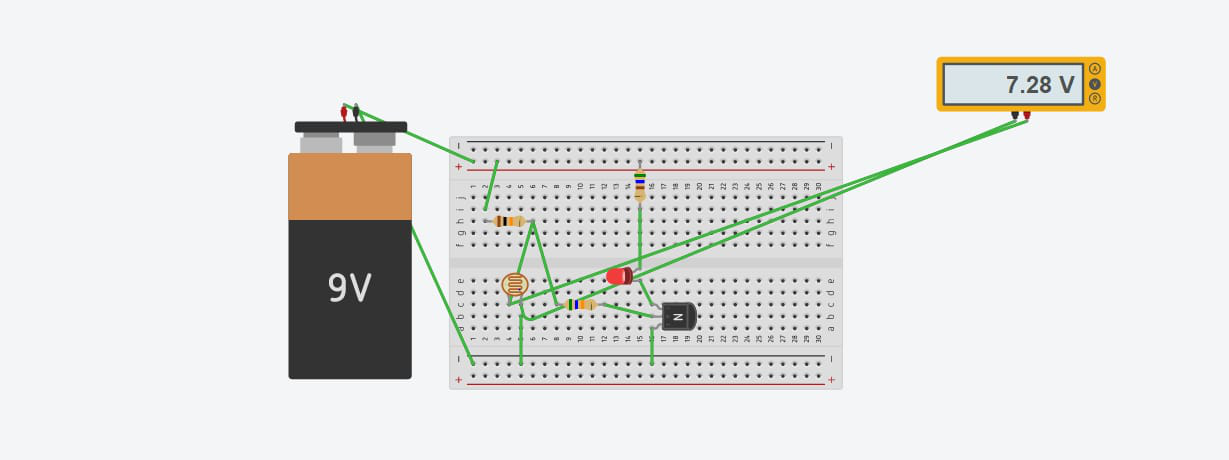
\includegraphics[width=12cm, height=5cm]{g11.png}

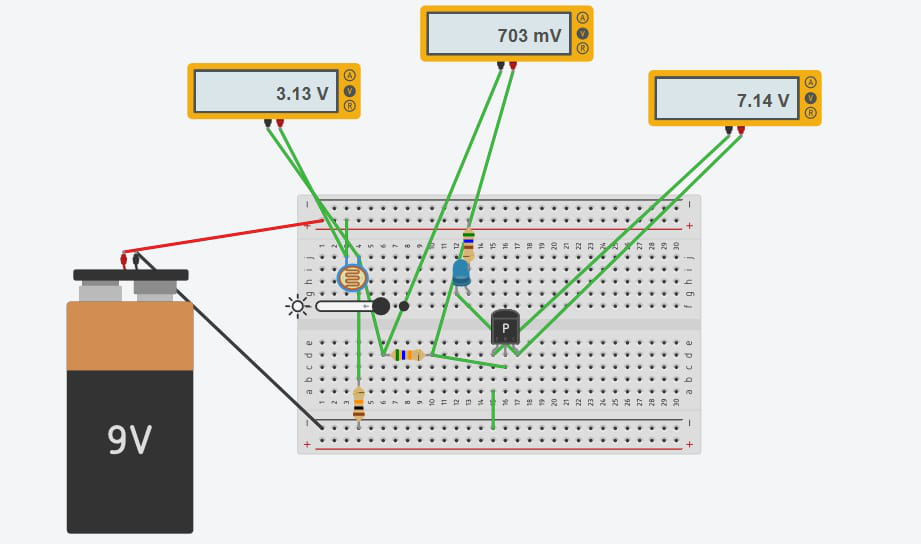
\includegraphics[width=12cm, height=6cm]{g12.png}

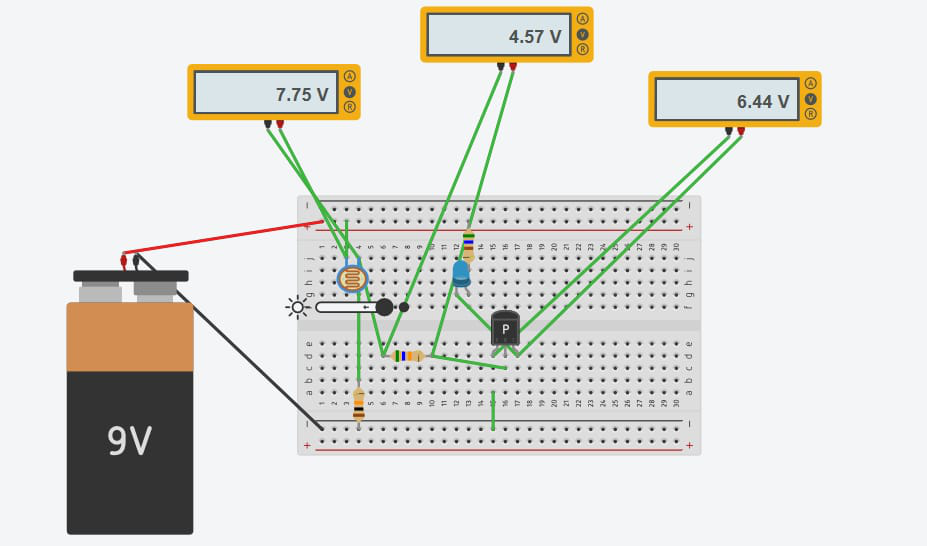
\includegraphics[width=12cm, height=6cm]{g13.png}
\end{center}
\end{figure}
\vspace{2cm}

\newpage
\begin{figure}
\paragraph{Gambar Hardware Rangkaian Komparator}
\paragraph{ }
\begin{center}

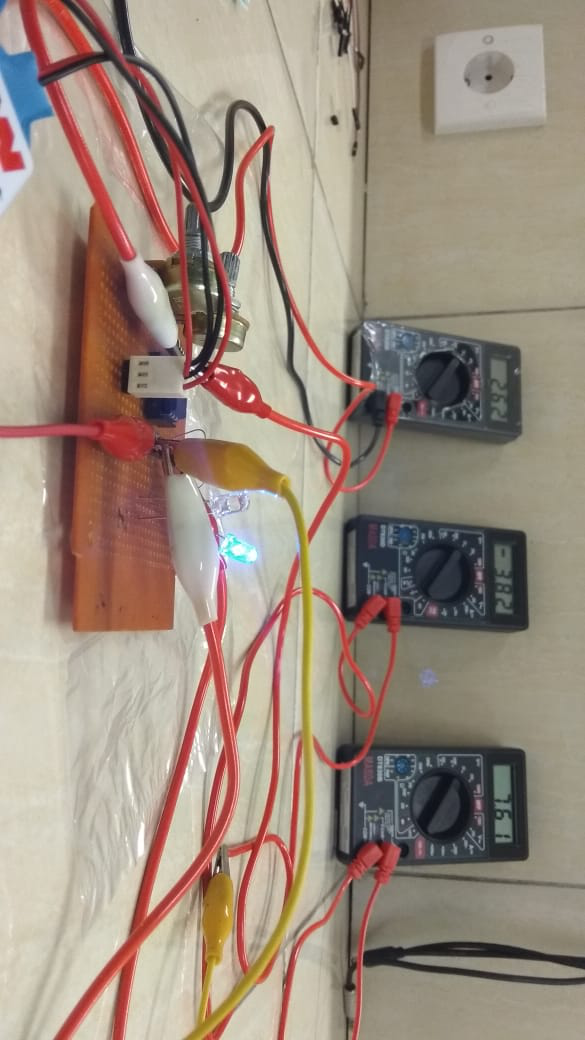
\includegraphics[width=7cm, height=12cm]{g1.png}

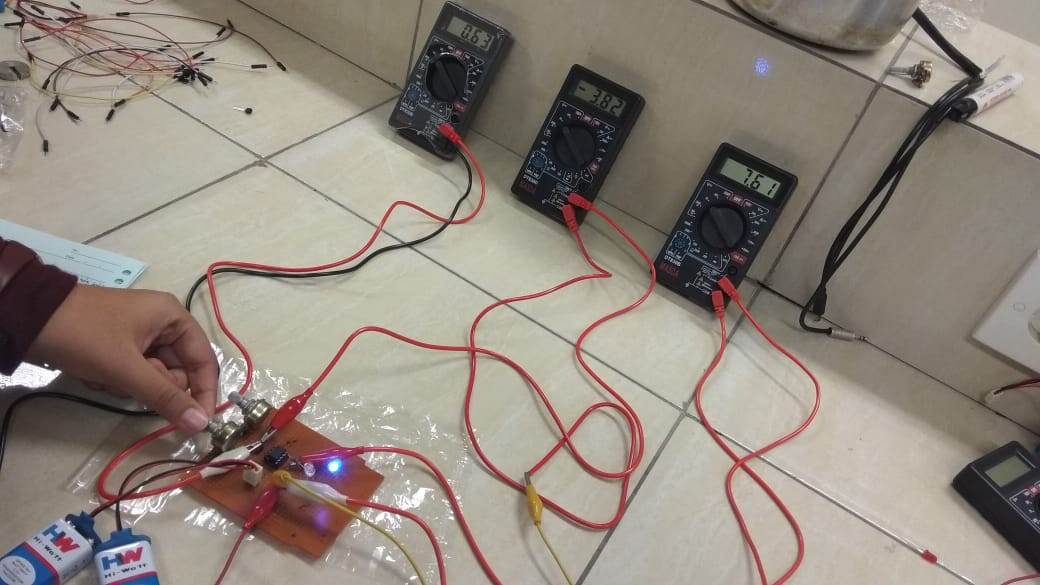
\includegraphics[width=12cm, height=6cm]{g2.png}

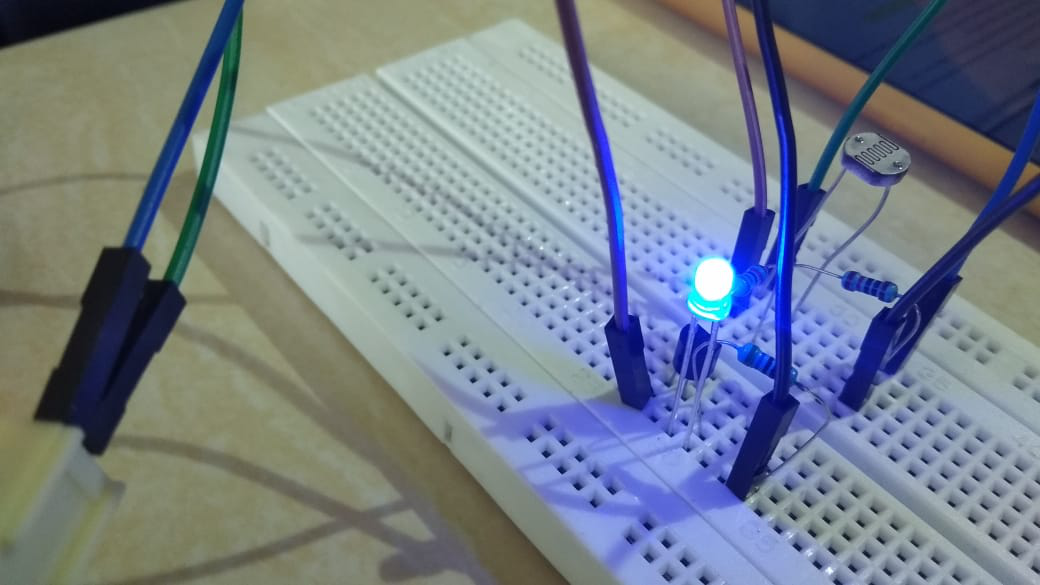
\includegraphics[width=12cm, height=6cm]{g3.png}
\end{center}
\end{figure}
\vspace{2cm}

\newpage
\begin{figure}
\paragraph{Gambar Hardware Rangkaian Transistor NPN}
\paragraph{ }
\begin{center}

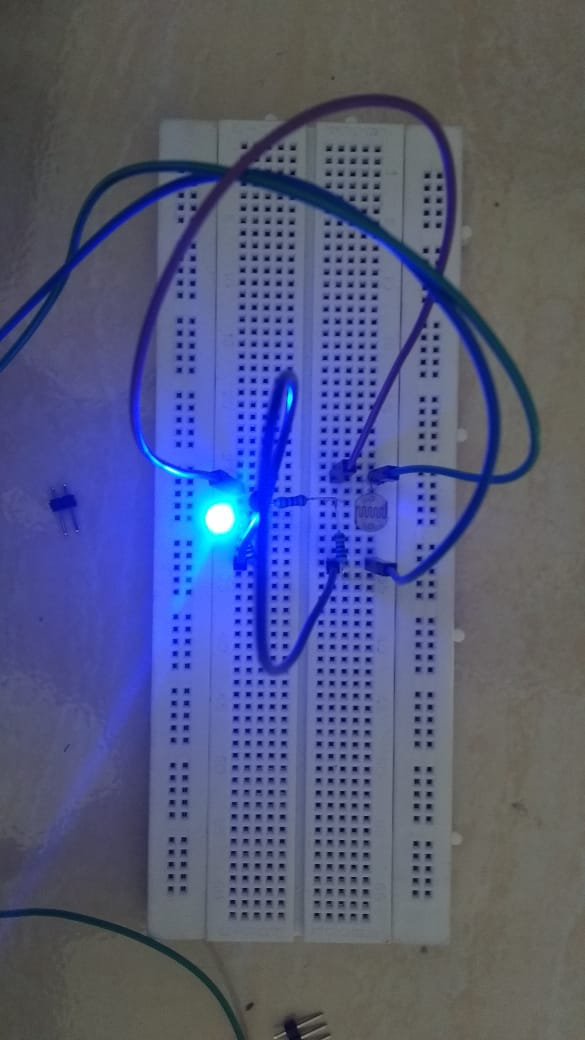
\includegraphics[width=7cm, height=12cm]{g4.png}

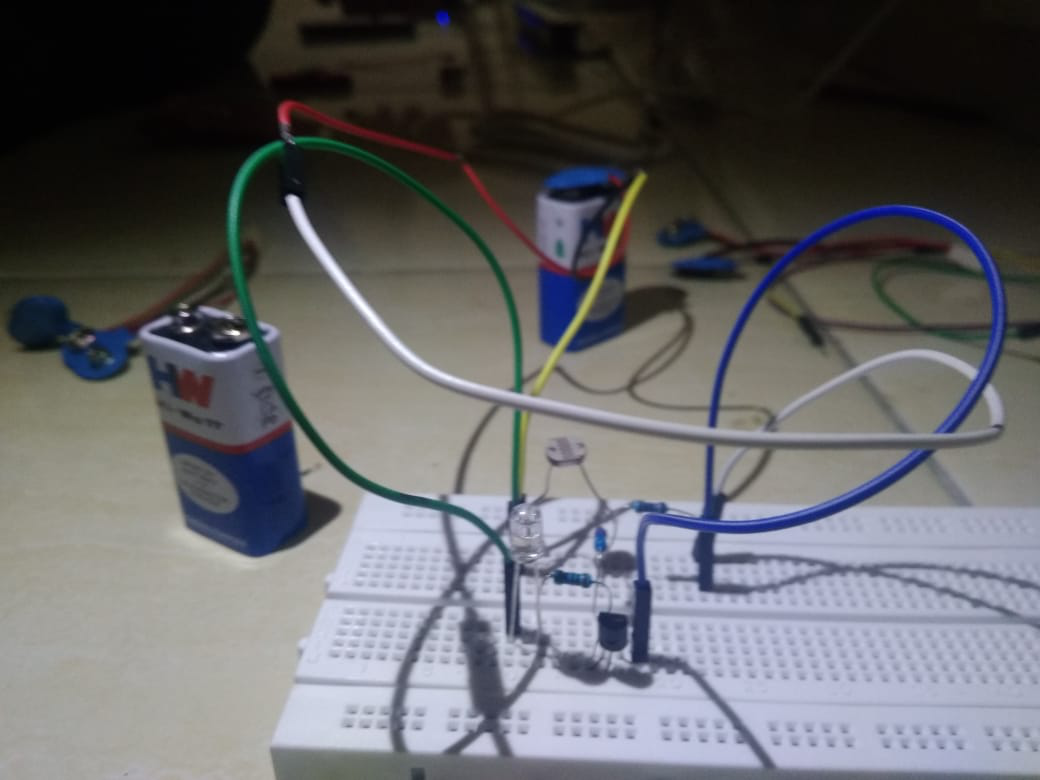
\includegraphics[width=12cm, height=6cm]{g5.png}

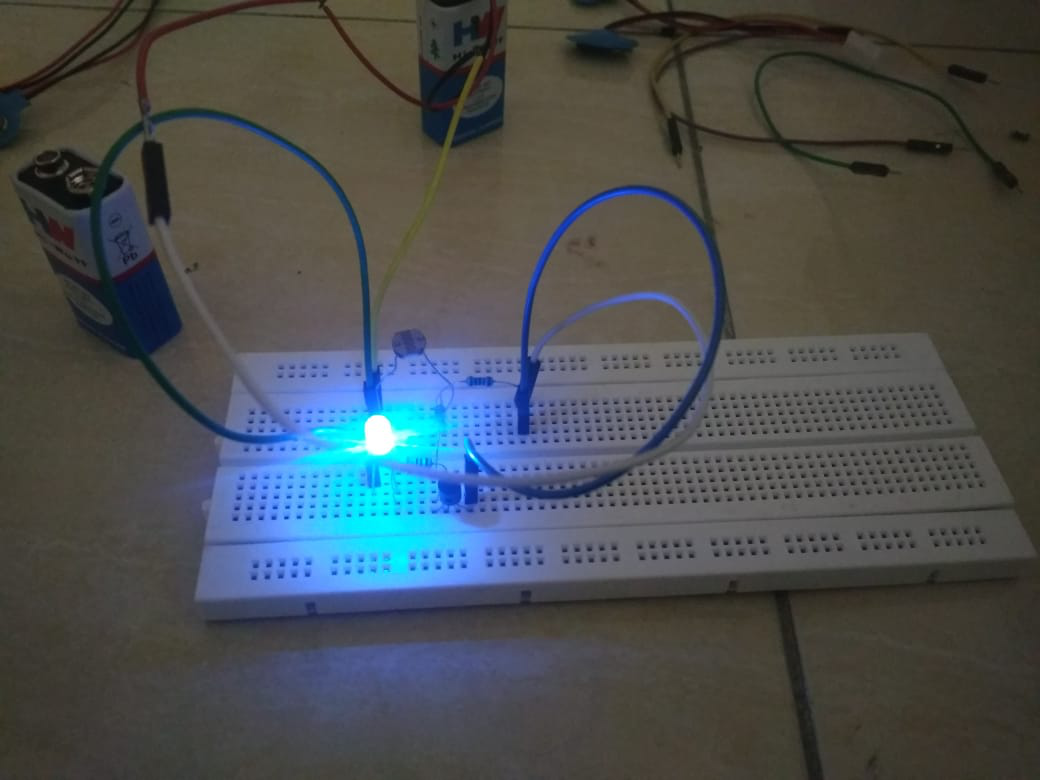
\includegraphics[width=12cm, height=6cm]{g6.png}
\end{center}
\end{figure}
\vspace{2cm}

\newpage
\begin{figure}
\paragraph{Gambar Hardware Rangkaian Transistor PNP}
\paragraph{ }
\begin{center}

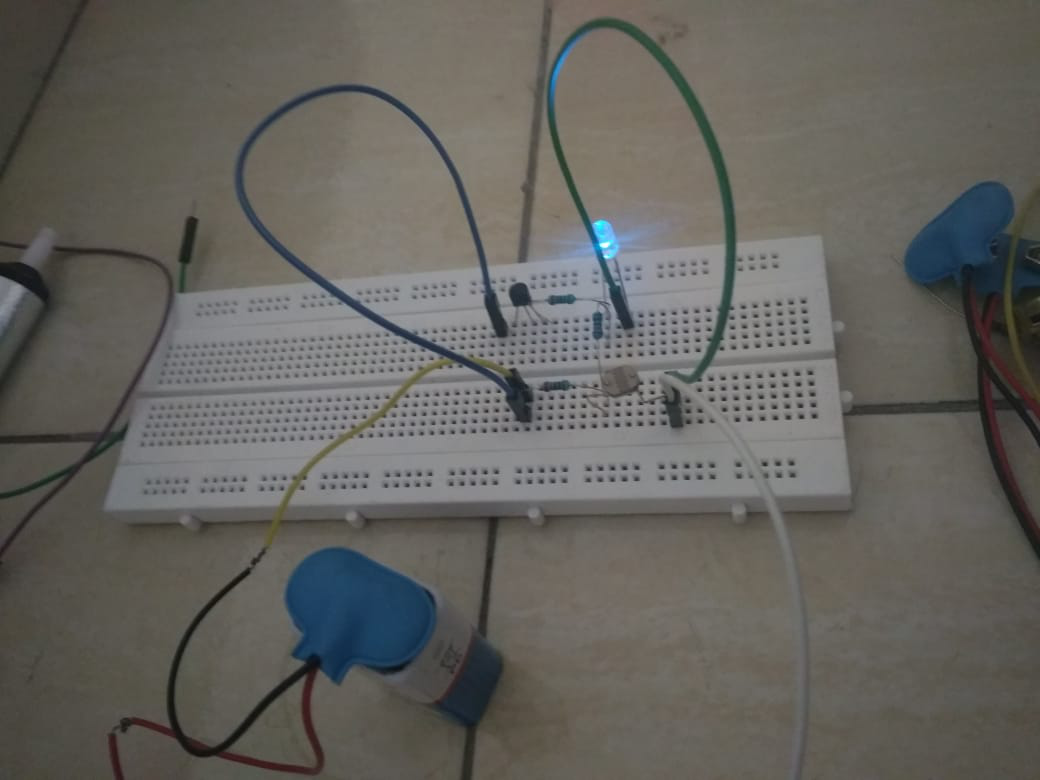
\includegraphics[width=7cm, height=12cm]{g7.png}

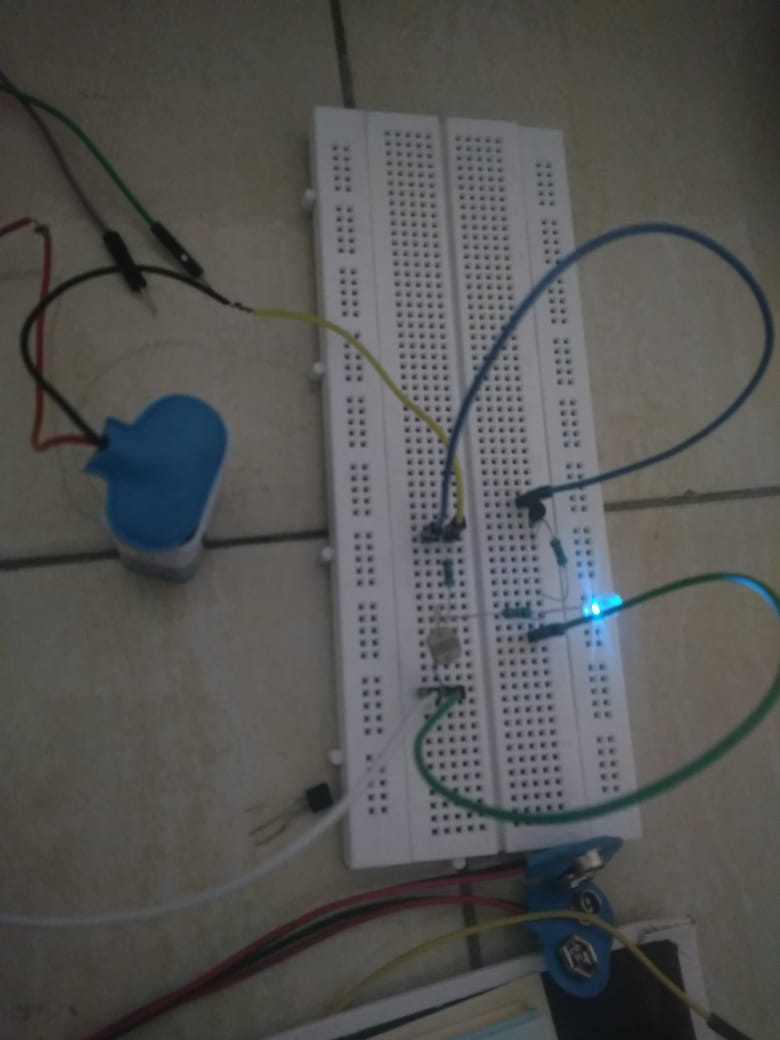
\includegraphics[width=12cm, height=6cm]{g8.png}

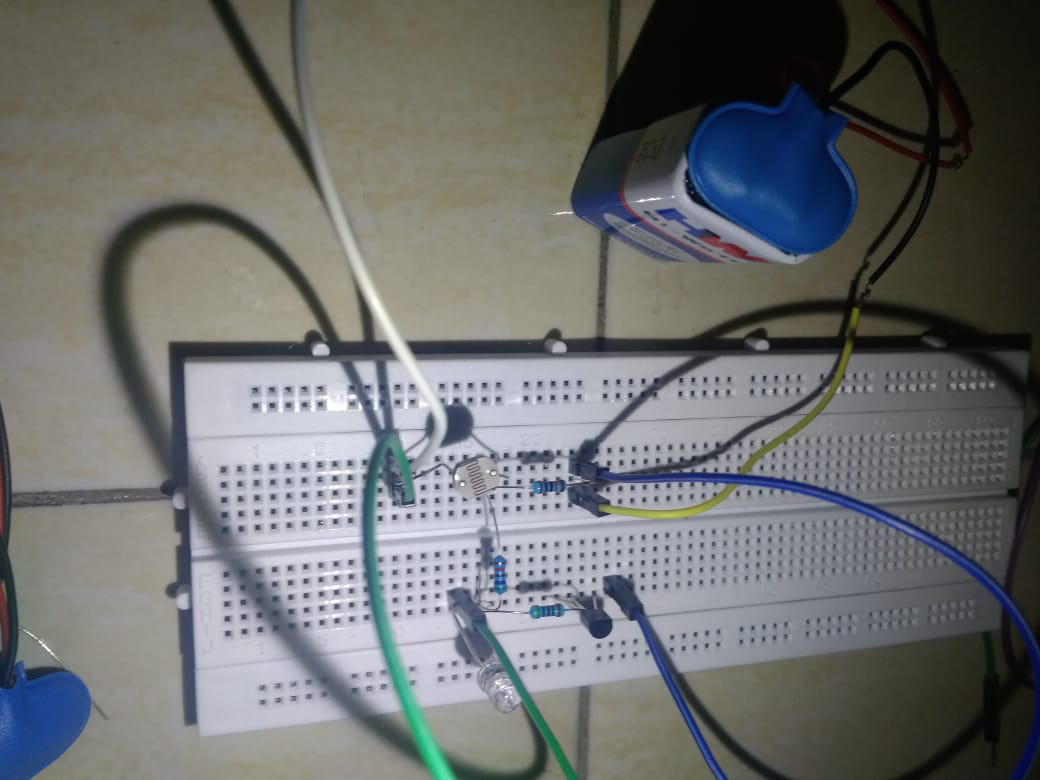
\includegraphics[width=12cm, height=6cm]{g9.png}
\end{center}
\end{figure}
\vspace{2cm}

\end{document} %Penulisan Laporan Berakhir
